% Este arquivo .tex será incluído no arquivo .tex principal. Não é preciso
% declarar nenhum cabeçalho

\section{Atlética -- AAACEC}

A \textbf{AAACEC -- Associação Atlética Acadêmica da Ciência e Engenharia de
Computação}, ou simplesmente \textbf{Atlética}, é a entidade estudantil que
promove a prática de esportes na Computação.

Uma entidade sem fins lucrativos, a AAACEC tem sua diretoria eleita anualmente
pel*s alun*s associad*s dos cursos de Engenharia e Ciência da Computação e da
pós-graduação no IC.

A Atlética é responsável pela participação da Computação em competições
esportivas, tanto dentro da Unicamp (Calouríadas, Interanos, Olimpíadas) quanto
fora (Intercomp).

\begin{figure}[H]
    \centering
    \includegraphics[scale=0.55]{img/alem_da_graduacao/aaacec_foto.jpg}
\end{figure}

A fim de possibilitar essa participação, a AAACEC promove treinos regulares de
basquete, vôlei, handebol e futsal e disponibiliza o material (bolas, redes
etc.) para a prática de tais esportes. A AAACEC se encarrega da reserva de
quadras para a realização dos treinos e competições em que isso se fizer
necessário. Os treinos são semanais e oferecidos para as modalidades masculina e
feminina, de forma que qualquer associad* da Atlética pode participar.

Para associar-se à AAACEC, *s ingressantes podem comprar o \textbf{Kit Bixo},
que contém produtos como camiseta, caneca, mouse pad e chaveiro. Veteran*s podem
associar-se mediante o pagamento de uma taxa. Além do Kit Bix*, a AAACEC vende
outros produtos, como agasalhos.

Além de promover a prática esportiva, a Atlética também realiza festas e eventos
de integração, como a tradicional \textbf{Choppada da Computação} no começo do
ano (gratuita para bix*s, não perca!).

Para saber mais sobre a Atlética e como participar, entre em contato por:

\begin{compactitemize}
\item  E-mail: \email{aaacec@gmail.com}
\item  Site: \url{aaacec.com}
\end{compactitemize}

\subsection{Bateria Valorosa}

\begin{figure}[H]
    \centering
    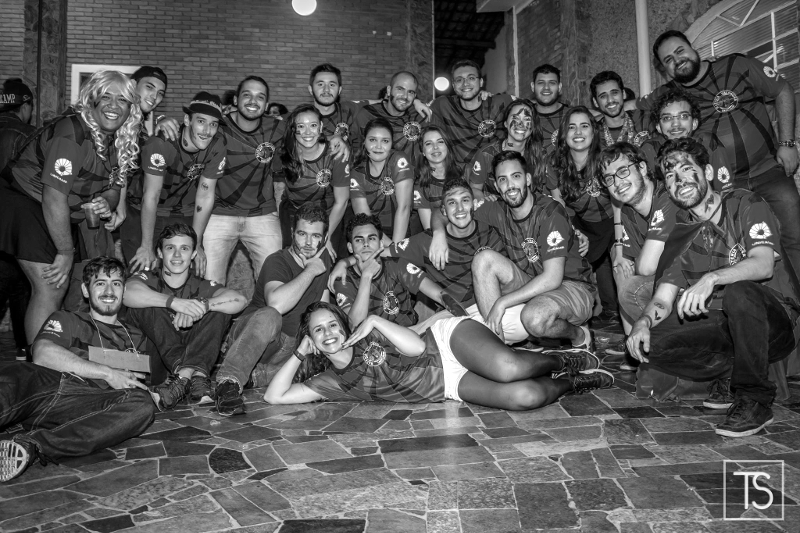
\includegraphics[scale=0.27]{img/alem_da_graduacao/valorosa_foto1.jpg}
\end{figure}

Criada em 1998 e filiada à AAACEC, a \textbf{Bateria Valorosa} é umas das
melhores baterias universitárias da Unicamp. Você muito provavelmente vai
conhecê-la no primeiro dia de aula.

Ao longo do ano, a Valorosa toca em diversos eventos, como o Intercomp, o
Interbatuc e a UPA. A Bateria toca também em festas e para apoiar *s atletas em
jogos internos da Computação e de outros cursos.

A Valorosa realiza ensaios semanais, dos quais estão tod*s, especialmente bix*s,
convidados a participar. Basta comparecer aos ensaios, não é necessário saber
tocar nenhum instrumento. Tod*s que quiserem aprender são muito bem-vind*s na
bateria!

Para mais informações sobre a Bateria Valorosa, acesse o site da AAACEC.

\begin{figure}[H]
    \centering
    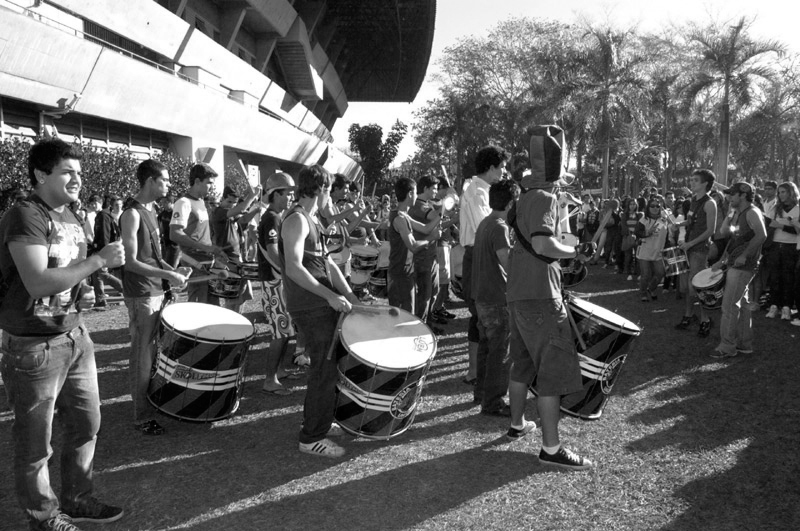
\includegraphics[scale=0.27]{img/alem_da_graduacao/valorosa_foto2.jpg}
\end{figure}
